\documentclass[a4paper,11pt]{book}
%\documentclass[a4paper,twoside,11pt,titlepage]{book}
\usepackage{listings}
\usepackage[utf8]{inputenc}
\usepackage[spanish]{babel}

% \usepackage[style=list, number=none]{glossary} %
%\usepackage{titlesec}
%\usepackage{pailatino}

\decimalpoint
\usepackage{dcolumn}
\newcolumntype{.}{D{.}{\esperiod}{-1}}
\makeatletter
\addto\shorthandsspanish{\let\esperiod\es@period@code}
\makeatother


%\usepackage[chapter]{algorithm}
\RequirePackage{verbatim}
%\RequirePackage[Glenn]{fncychap}
\usepackage{fancyhdr}
\usepackage{graphicx}
\usepackage{afterpage}

\usepackage{longtable}

\usepackage[pdfborder={000}]{hyperref} %referencia

% ********************************************************************
% Re-usable information
% ********************************************************************
\newcommand{\myTitle}{Título del proyecto\xspace}
\newcommand{\myDegree}{Máster Universitario en Desarrollo de Software\xspace}
\newcommand{\myName}{Nombre Apllido1 Apellido2 (alumno)\xspace}
\newcommand{\myProf}{Nombre Apllido1 Apellido2 (tutor1)\xspace}
\newcommand{\myOtherProf}{Nombre Apllido1 Apellido2 (tutor2)\xspace}
%\newcommand{\mySupervisor}{Put name here\xspace}
\newcommand{\myFaculty}{Escuela Técnica Superior de Ingenierías Informática y de
Telecomunicación\xspace}
\newcommand{\myFacultyShort}{E.T.S. de Ingenierías Informática y de
Telecomunicación\xspace}
\newcommand{\myDepartment}{Departamento de Lenguajes y Sistemas Informáticos\xspace}
\newcommand{\myUni}{\protect{Universidad de Granada}\xspace}
\newcommand{\myLocation}{Granada\xspace}
\newcommand{\myTime}{\today\xspace}
\newcommand{\myVersion}{Version 0.1\xspace}


\hypersetup{
pdfauthor = {\myName (email (en) ugr (punto) es)},
pdftitle = {\myTitle},
pdfsubject = {},
pdfkeywords = {palabra_clave1, palabra_clave2, palabra_clave3, ...},
pdfcreator = {LaTeX con el paquete ....},
pdfproducer = {pdflatex}
}

%\hyphenation{}


%\usepackage{doxygen/doxygen}
%\usepackage{pdfpages}
\usepackage{url}
\usepackage{colortbl,longtable}
\usepackage[stable]{footmisc}
%\usepackage{index}

%\makeindex
%\usepackage[style=long, cols=2,border=plain,toc=true,number=none]{glossary}
% \makeglossary

% Definición de comandos que me son tiles:
%\renewcommand{\indexname}{Índice alfabético}
%\renewcommand{\glossaryname}{Glosario}

\pagestyle{fancy}
\fancyhf{}
\fancyhead[LO]{\leftmark}
\fancyhead[RE]{\rightmark}
\fancyhead[RO,LE]{\textbf{\thepage}}
\renewcommand{\chaptermark}[1]{\markboth{\textbf{#1}}{}}
\renewcommand{\sectionmark}[1]{\markright{\textbf{\thesection. #1}}}

\setlength{\headheight}{1.5\headheight}

\newcommand{\HRule}{\rule{\linewidth}{0.5mm}}
%Definimos los tipos teorema, ejemplo y definición podremos usar estos tipos
%simplemente poniendo \begin{teorema} \end{teorema} ...
\newtheorem{teorema}{Teorema}[chapter]
\newtheorem{ejemplo}{Ejemplo}[chapter]
\newtheorem{definicion}{Definición}[chapter]

\definecolor{gray97}{gray}{.97}
\definecolor{gray75}{gray}{.75}
\definecolor{gray45}{gray}{.45}
\definecolor{gray30}{gray}{.94}

\lstset{ frame=Ltb,
     framerule=0.5pt,
     aboveskip=0.5cm,
     framextopmargin=3pt,
     framexbottommargin=3pt,
     framexleftmargin=0.1cm,
     framesep=0pt,
     rulesep=.4pt,
     backgroundcolor=\color{gray97},
     rulesepcolor=\color{black},
     %
     stringstyle=\ttfamily,
     showstringspaces = false,
     basicstyle=\scriptsize\ttfamily,
     commentstyle=\color{gray45},
     keywordstyle=\bfseries,
     %
     numbers=left,
     numbersep=6pt,
     numberstyle=\tiny,
     numberfirstline = false,
     breaklines=true,
   }
 
% minimizar fragmentado de listados
\lstnewenvironment{listing}[1][]
   {\lstset{#1}\pagebreak[0]}{\pagebreak[0]}

\lstdefinestyle{CodigoC}
   {
	basicstyle=\scriptsize,
	frame=single,
	language=C,
	numbers=left
   }
\lstdefinestyle{CodigoC++}
   {
	basicstyle=\small,
	frame=single,
	backgroundcolor=\color{gray30},
	language=C++,
	numbers=left
   }

 
\lstdefinestyle{Consola}
   {basicstyle=\scriptsize\bf\ttfamily,
    backgroundcolor=\color{gray30},
    frame=single,
    numbers=none
   }


\newcommand{\bigrule}{\titlerule[0.5mm]}


%Para conseguir que en las páginas en blanco no ponga cabecerass
\makeatletter
\def\clearpage{%
  \ifvmode
    \ifnum \@dbltopnum =\m@ne
      \ifdim \pagetotal <\topskip
        \hbox{}
      \fi
    \fi
  \fi
  \newpage
  \thispagestyle{empty}
  \write\m@ne{}
  \vbox{}
  \penalty -\@Mi
}
\makeatother

\usepackage{pdfpages}
\begin{document}
\begin{titlepage}
 
 
\newlength{\centeroffset}
\setlength{\centeroffset}{-0.5\oddsidemargin}
\addtolength{\centeroffset}{0.5\evensidemargin}
\thispagestyle{empty}

\noindent\hspace*{\centeroffset}\begin{minipage}{\textwidth}

\centering

\includegraphics[width=0.9\textwidth]{imagenes/logo_ugr.jpg}\\[1.4cm]

\textsc{ \Large TRABAJO FIN DE MÁSTER\\[0.2cm]}
\textsc{ MÁSTER UNIVERSITARIO EN ANTROPOLOGÍA FÍSICA Y FORENSE}\\[1cm]
% Upper part of the page
% 
% Title
{\Huge\bfseries Daño Axonal Difuso\\
}
\noindent\rule[-1ex]{\textwidth}{3pt}\\[3.5ex]
{\large\bfseries La marca de los traumatismos craneoencefálicos}
\end{minipage}

\vspace{2.5cm}
\noindent\hspace*{\centeroffset}\begin{minipage}{\textwidth}
\centering

\textbf{Autor}\\ {Adela Sabio González}\\[2.5ex]
\textbf{Directores}\\
{María Inmaculada Alemán Aguilera\\
Elisa María Cabrerizo Medina}\\[2cm]

\includegraphics[width=0.3\textwidth]{imagenes/etsiit_logo.png}\\[0.1cm]
\textsc{Facultad de Medicina}\\
\textsc{---}\\
Granada, octubre de 2018
\end{minipage}
%\addtolength{\textwidth}{\centeroffset}
%\vspace{\stretch{2}}
\end{titlepage}



\chapter*{}
%\thispagestyle{empty}
%\cleardoublepage

%\thispagestyle{empty}

\begin{titlepage}
 
 
\setlength{\centeroffset}{-0.5\oddsidemargin}
\addtolength{\centeroffset}{0.5\evensidemargin}
\thispagestyle{empty}

\noindent\hspace*{\centeroffset}\begin{minipage}{\textwidth}

\centering
%
\includegraphics[width=0.9\textwidth]{imagenes/logo_ugr.jpg}\\[1.4cm]

%\textsc{ \Large PROYECTO FIN DE CARRERA\\[0.2cm]}
%\textsc{ INGENIERÍA EN INFORMÁTICA}\\[1cm]
% Upper part of the page
% 

 \vspace{3.3cm}

%si el proyecto tiene logo poner aquí

\includegraphics{imagenes/logo.png} 
 \vspace{0.5cm}

% Title

{\Huge\bfseries Título del proyecto\\
}
\noindent\rule[-1ex]{\textwidth}{3pt}\\[3.5ex]
{\large\bfseries Subtítulo del proyecto.\\[4cm]}
\end{minipage}

\vspace{2.5cm}
\noindent\hspace*{\centeroffset}\begin{minipage}{\textwidth}
\centering

\textbf{Autor}\\ {Nombre Apellido1 Apellido2 (alumno)}\\[2.5ex]
\textbf{Directores}\\
{Nombre Apellido1 Apellido2 (tutor1)\\
Nombre Apellido1 Apellido2 (tutor2)}\\[2cm]
%
\includegraphics[width=0.15\textwidth]{imagenes/tstc.png}\\[0.1cm]
%\textsc{Departamento de Teoría de la Señal, Telemática y Comunicaciones}\\
%\textsc{---}\\
%Granada, mes de 201
\end{minipage}
%\addtolength{\textwidth}{\centeroffset}
\vspace{\stretch{2}}

 
\end{titlepage}






\cleardoublepage
\thispagestyle{empty}

\begin{center}
{\large\bfseries Título del Proyecto: Subtítulo del proyecto}\\
\end{center}
\begin{center}
Nombre Apellido1 Apellido2 (alumno)\\
\end{center}

%\vspace{0.7cm}
\noindent{\textbf{Palabras clave}: palabra\_clave1, palabra\_clave2, palabra\_clave3, ......}\\

\vspace{0.7cm}
\noindent{\textbf{Resumen}}\\

Poner aquí el resumen.
\cleardoublepage


\thispagestyle{empty}


\begin{center}
{\large\bfseries Project Title: Project Subtitle}\\
\end{center}
\begin{center}
First name, Family name (student)\\
\end{center}

%\vspace{0.7cm}
\noindent{\textbf{Keywords}: Keyword1, Keyword2, Keyword3, ....}\\

\vspace{0.7cm}
\noindent{\textbf{Abstract}}\\

Write here the abstract in English.

\chapter*{}
\thispagestyle{empty}

\noindent\rule[-1ex]{\textwidth}{2pt}\\[4.5ex]

Yo, \textbf{Nombre Apellido1 Apellido2}, alumno del \textbf{Máster en Desarrollo de Software} de la \textbf{Escuela Técnica Superior
de Ingenierías Informática y de Telecomunicación de la Universidad de Granada}, con DNI XXXXXXXXX, autorizo la
ubicación de la siguiente copia de mi Trabajo Fin de Máster en la biblioteca del centro para que pueda ser
consultada por las personas que lo deseen.

\vspace{6cm}

\noindent Fdo: Nombre Apellido1 Apellido2

\vspace{2cm}

\begin{flushright}
Granada a X de mes de 201 .
\end{flushright}


\chapter*{}
\thispagestyle{empty}

\noindent\rule[-1ex]{\textwidth}{2pt}\\[4.5ex]

D. \textbf{Nombre Apellido1 Apellido2 (tutor1)}, Profesor del Área de XXXX del Departamento YYYY de la Universidad de Granada.

\vspace{0.5cm}

D. \textbf{Nombre Apellido1 Apellido2 (tutor2)}, Profesor del Área de XXXX del Departamento YYYY de la Universidad de Granada.


\vspace{0.5cm}

\textbf{Informan:}

\vspace{0.5cm}

Que el presente trabajo, titulado \textit{\textbf{Título del proyecto, Subtítulo del proyecto}},
ha sido realizado bajo su supervisión por \textbf{Nombre Apellido1 Apellido2 (alumno)}, y autorizamos la defensa de dicho trabajo ante el tribunal
que corresponda.

\vspace{0.5cm}

Y para que conste, expiden y firman el presente informe en Granada a X de mes de 201 .

\vspace{1cm}

\textbf{Los directores:}

\vspace{5cm}

\noindent \textbf{Nombre Apellido1 Apellido2 (tutor1) \ \ \ \ \ Nombre Apellido1 Apellido2 (tutor2)}


\chapter*{}
\thispagestyle{empty}

\noindent\rule[-1ex]{\textwidth}{2pt}\\[4.5ex]

Yo, \textbf{Nombre Apellido1 Apellido2}, alumno del \textbf{Máster en Desarrollo de Software} de la \textbf{Escuela Técnica Superior
de Ingenierías Informática y de Telecomunicación de la Universidad de Granada}, con DNI XXXXXXXXX, \underline{declaro explícitamente} que el trabajo presentado es original, entendido en el sentido que no he utilizado ninguna fuente sin citarla debidamente.

\vspace{6cm}

\noindent Fdo: Nombre Apellido1 Apellido2

\vspace{2cm}

\begin{flushright}
Granada a X de mes de 201 .
\end{flushright}


\chapter*{Agradecimientos}
\thispagestyle{empty}

       \vspace{1cm}


Poner aquí agradecimientos...


%\frontmatter
%\tableofcontents
%\listoffigures
%\listoftables
%
%\mainmatter
%\setlength{\parskip}{5pt}

\chapter{Introducción}
La evaluación forense es un trabajo en equipo en el que intervienen múltiples expertos con el fin de determinar los procesos que llevaron a la muerte de un individuo. Entre ellos, cabe destacar la importancia de la unión entre el antropólogo forense, el médico forense y el histopatólogo forense, ya que las lesiones que identifica el primero permiten al segundo establecer el contexto clínico-patológico en el que tuvieron lugar, siendo confirmados (en los casos en los que sea posible) por el último. De esa interacción nace este estudio, orientado a establecer la data y causa de muerte en los frecuentes casos de contusión craneal traumática, que no siempre dan lugar a una lesión evidente que justifique la muerte de la víctima.\ 
En primer lugar, se procederá a realizar una revisión sobre las lesiones craneales asociadas a contusiones, y la importancia del antropólogo forense en su evaluación. A continuación, se hará un breve resumen sobre las lesiones encefálicas asociadas a las mismas, dando lugar finalmente a la descripción de nuestro estudio, con los antecedentes del mismo, los métodos empleados para realizarlo, y los resultados preliminares, con vistas a continuarlo en un futuro.\ 

\section{Lesiones craneales asociadas a contusiones} \cite{Finnie2016} \cite{Kranioti2015} \cite{Sulaiman2014}
La antropología forense es una disciplina complementaria a la patología forense en el examen de restos óseos, cuyo fin es determinar la etiología médico-legal de la muerte, la causa de la misma y sus mecanismos de producción. Del antropólogo forense depende el análisis de las lesiones óseas, al que se le solicita que evalúe su data, que identifique patrones traumáticos y que trate de determinar el objeto lesivo (si lo hay), de tal manera que pueda concluir si esa lesión tiene que ver o no con la muerte del individuo. Si la lesión está en relación con la muerte, el antropólogo forense intentará aportar datos sobre si la etiología es violenta, y, en este caso, buscará encuadrar la etiología médico-legal como accidental, suicida u homicida.\ 
Los traumatismos por contusión se definen como lesiones producidas por la acción de cuerpos duros, romos (sin bordes cortantes) que actúan sobre el organismo por intermedio de una fuerza más o menos considerable.\
\section{Estableciendo la data}
La primera cuestión a abordar es la data de las lesiones, para determinar si coinciden o están en relación con la causa de la muerte. Se definen como antemortem, perimortem o posmortem.\
\begin{itemize}
	\item Antemortem (previas a la muerte): En este tipo de lesiones, hay evidencia de curación, en forma de signos de remodelación, osteofitos y/ó formación de callo ó puentes óseos. Sin embargo, hay que tener en cuenta que tardan en aparecer 1-3 semanas (la calcificación aparece a partir de la tercera semana).  El tipo de remodelación depende del hueso, los huesos largos tienden a formar callo, mientras que el cráneo desarrolla puentes óseos \cite{Kranioti2015}
	\item Perimortem (alrededor de la muerte): este término puede inducir a confusión si no se determina si nos estamos refiriendo al término médico legal (alrededor del momento de la muerte, asociado probablemente a la causa de la misma) ó al término antropológico-forense (considera que tienen lugar cuando el hueso todavía muestra propiedades viscoelásticas, antes de entrar en estado “seco” - que varía según la parte del cuerpo-) \cite{Kranioti2015}
	\item Postmortem (posteriores a la muerte): son el resultado de alteraciones tafonómicas o de recolección ósea. 
\end{itemize}
El mayor reto a la hora de establecer la data aparece a la hora de determinar si las lesiones son perimortem ó postmortem, ya que tras la muerte el hueso puede conservar temporalmente parte de sus propiedades viscoelásticas. En la siguiente tabla, elaborada por Kranioti\cite{Kranioti2015}, se proponen una serie de criterios para diferenciar el momento de producción de la lesión.\
Las fracturas tienden a migrar hacia la zona estructuralmente más débil de cráneo (como en las que hay abundancia de vasos). Si no se observan señales de curación, es muy posible que dichas lesiones estén en relación con la muerte. 
\subsection{Clasificación de las lesiones}
Las fracturas tienden a migrar hacia la zona estructuralmente más débil de cráneo (como en las que hay abundancia de vasos). Si no se observan señales de curación, es muy posible que dichas lesiones estén en relación con la muerte.

\begin{figure}
	\centering
	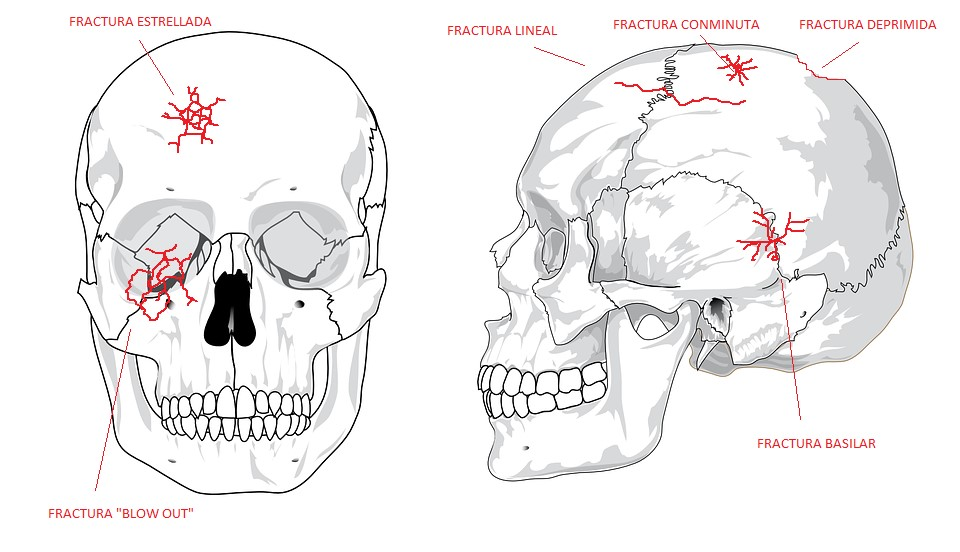
\includegraphics[width=0.7\textwidth]{imagenes/Figura1}
	\caption{Tipos de fracturas}
	\label{fig:figura1}
\end{figure}

\begin{itemize}
	\item Fracturas lineales: incluyen las fisuras, que aparecen principalmente en la bóveda craneal, las fracturas basilares (afectan a la base del cráneo) y las fracturas diastáticas (separación de suturas preexistentes). 
	\item Fracturas deprimidas: se producen por la aplicación de una carga intensa, lenta, en un área reducida del cráneo, provocando múltiples líneas de fractura (conminuta) en la superficie. Los fragmentos generados se deprimen o extienden en el encéfalo.  Dentro de las mismas, distinguimos: 
	\begin{itemize}
		\item Fracturas estrelladas, en las que el fragmento óseo del lugar del impacto se deprime y la periferia se sobreeleva, dando lugar al patrón característico de fracturas concéntricas cruzadas por fracturas lineales.
		\item Fracturas en estanque, que son fracturas profundas, deprimidas, resultado de compresión o continuación de una fractura lineal.
		\item Fracturas en anillo, que consisten en fracturas circulares alrededor del foramen magno, resultado de una fuerza que comprime la cabeza contra la columna. Son propias de las caídas de pie o de nalgas, o en accidentes en los que la cabeza del conductor impacta primero, forzando el cráneo contra la columna. 
		\end{itemize}
	\item Fractura orbitaria (“blowout”).
	\item Fracturas faciales: siguiendo la clasificación de Le Fort \ref{fig:figura2}, se distinguen 3 tipos:
	\begin{itemize}
		\item Le Fort I: o transversal de maxilar superior: la línea de fractura es horizontal, se localiza sobre los ápices dentarios y se extiende hasta las apófisis pterigoides, afectando al hueso palatino. 
		\item Le Fort II o piramidal: es una fractura en forma de pirámide que compromete huesos propios, proceso ascendente del maxilar, reborde orbitario y desciende siguiendo una trayectoria similar a la tipo I. 
		\item Le Fort III o disyunción cráneo facial: el cráneo se separa del macizo facial. Se produce cuando la fuerza traumática del impacto es suficiente para separar todos los huesos de la cara de sus uniones con la base del cráneo.
	\end{itemize}

\begin{figure}
	\centering
	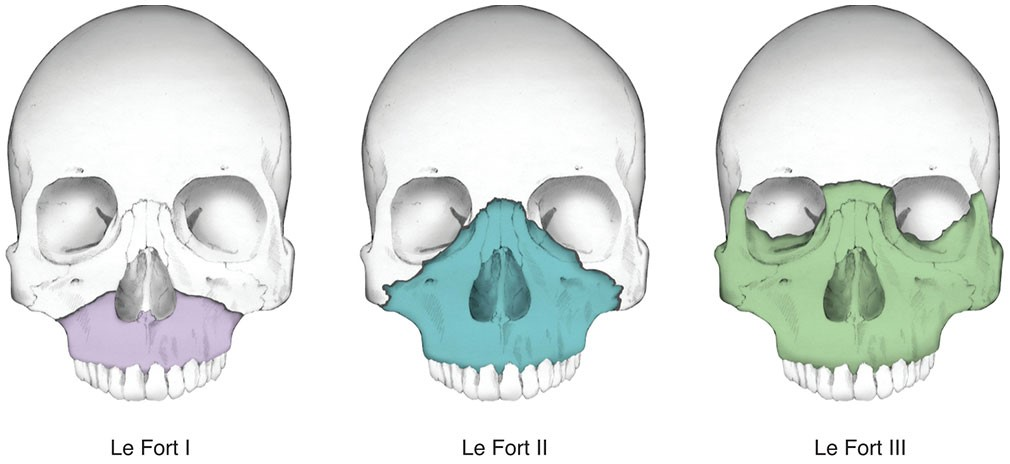
\includegraphics[width=0.7\textwidth]{imagenes/Figura2}
	\caption{Clasificación de Le Fort}
	\label{fig:figura2}
\end{figure}

	\item Fractura contragolpe: fractura distante del punto en el que se originó el traumatismo. 
	\item Hay casos en los que las fracturas dejan la tabla externa intacta mientras que la interna se rompe, dañando el cerebro. 
\end{itemize}
\subsection{Determinando etiología}
Las lesiones craneales son las causas de muerte mecánica más comunes implicadas en accidentes de tráfico, suicidio (precipitación) y violencia interpersonal. A la hora de analizarlas, hay que tener en cuenta que lesiones similares pueden producirse por distintos mecanismos y que el mismo mecanismo puede producir distintos patrones.
 
El tipo más común de lesión es la fractura lineal (70-80), asociada a caídas. Las fracturas deprimidas muestran una mayor correlación con violencia interpersonal, como, por ejemplo, asalto con un bate de baseball (lesiones en bóveda craneal y fracturas lineales en base)\cite{Kranioti2015}
En el caso de que la cabeza pueda moverse con total libertad, las fracturas tienden a ser lineales o con depresión incompleta. Sin embargo, si la cabeza está inmóvil, suelen producirse fracturas conminuta.\cite{Tong2004}

Para diferenciar entre asalto violento o accidente, una de las primeras reglas que se propusieron fue la “hat brim line rule”, en la que, a partir de la máxima circunferencia de la bóveda, se consideraba que lesiones por encima de la misma son más propias de asalto, mientras que las lesiones inferiores son más propias de caída. Se observó que esta regla, en ausencia de otros criterios, no podía emplearse de manera sistemática, ya que con frecuencia originaba errores a la hora de establecer la etiología. Para paliar sus defectos, se propusieron otros criterios, como la lateralización, las laceraciones, abrasiones, presencia/ausencia de fracturas faciales, presencia/ausencia de traumatismos viscerales...

La lateralización tiene en cuenta el tipo de fractura y su localización. Por ejemplo, las fracturas lineales derechas son más frecuentes en las caídas, porque la población es predominantemente diestra, e intentan evitar la caída con el brazo derecho, haciendo que el cuerpo se incline hacia ese lado. Las fracturas lineales izquierdas, en cambio, suelen producirse en casos de asaltos de frente por agresores diestros. Una fractura deprimida posterior del cráneo hace pensar en un asaltante diestro localizado posterior a la víctima\cite{Kranioti2015}

Las fracturas craneales son más propias de caídas sobre tierra firme, mientras que las lesiones abdominales se asocian más a caídas en agua. Las fracturas faciales son más frecuentes en los casos de suicidio\cite{Kranioti2015}

Como factor altamente indicativo de homicidio, se considera la laceración roma, la contusión profunda o el traumatismo intracraneal, siendo este último el factor discriminatorio más relevante para diferenciar caída de homicidio, aunque no hay diferencias estadísticamente significativas entre los dos grupos basándose en el tipo de lesión (hematoma subdural ó extradural, contusión cerebral, hemorragia subaracnoidea y lesión axonal difusa)\cite{Kranioti2015}. Por último, hay que tener en cuenta que la presencia de múltiples lesiones en una misma ubicación o cercana a la misma, se asocia con más frecuencia a eventos violentos.

\subsection{Práctica actual}\cite{Kranioti2015} \cite{Traumatic}
Es muy frecuente que en las autopsias de individuos cuya muerte se deba a colisiones, accidentes, suicidios u homicidios se observen lesiones óseas, siendo la más común - sobre todo en homicidios- los traumatismos contusos en la cabeza. Es por ello que hay que establecer un protocolo sistematizado de trabajo que permita analizar todas las lesiones, de forma que facilite su posterior análisis y correlación.\
En primer lugar, se debe realizar una inspección de las lesiones en piel y partes blandas. Para ello, se emplean herramientas como la radiografía, la disección macroscópica y posterior análisis microscópico. Últimamente se plantea la posibilidad de realizar un TAC, con el fin de estudiar las partes blandas sin alteraciones asociadas a las mismas vinculadas a la manipulación (sin embargo, su elevado coste hace que sea una técnica restringida a casos particulares). El cuero cabelludo es una localización anatómica ideal para el desarrollo de abrasiones, contusiones y laceraciones debido a la presencia de partes blandas recubriendo las prominencias redondeadas del cráneo. El pelo, dependiendo de su espesor, puede producir una cierta protección y enmascarar abrasiones y contusiones. Las abrasiones de impactos occipitales y parietales pueden pasar desapercibidas sin una inspección adecuada y el cuidadoso afeitado de la zona de áreas en las que se sospeche traumatismo craneal. Determinar los puntos de impacto es importante para comparar la información aportada por testigos visuales ó correlacionar lesiones cerebrales subyacentes. Por lo tanto, es recomendable documentarlas con fotografías, diagramas y medidas. La evaluación histológica permite establecer la data y buscar fragmentos de restos óseos o de otros materiales. Por último, su forma y tamaño puede dar pistas sobre un posible instrumento usado por el agresor.

El siguiente paso, una vez liberada la calota, es observar la superficie ectocraneal, los bordes de los fragmentos y el ángulo de las fracturas lineales. En el caso de que haya múltiples fracturas, se recomienda hacer fotos y un dibujo, incluyendo las medidas de las fracturas y el empleo de descripciones anatómicas universales.\ 
En el caso de que las fracturas parezcan mostrar la huella de algún tipo de herramienta, no se ha de encajar directamente, ýa que puede alterar la distribución de la fractura. Es más recomendable hacer una comparación y realizar una sugerencia sobre el posible mecanismo de producción de la fractura.

Si bien los protocolos cambian según el centro de trabajo, se ha de intentar emplear un método fiable, repetible y aceptable, con tasas de error conocidas, que den un cierto grado de confianza y que puedan hacer frente a las exigencias del sistema judicial.

\section{Contusión craneal traumática y lesión encefálica}
Dentro del ámbito de la práctica forense, es común encontrarse con muertes de causa desconocida, en las que una buena práctica consiste en examinar el cerebro en busca de patrones de lesión cerebral que sugieran un traumatismo, ya sean focales (fracturas, hematomas, contusiones) ó difusas (isquemia global, edema cerebral y lesión axonal difusa traumática).

La lesión cerebral traumática se conoce como la “epidemia silenciosa” y supone aproximadamente un 1-2 de las muertes de cualquier causa, constituyendo de un tercio a la mitad de las muertes asociadas a traumatismos1. Las principales lesiones asociadas a traumatismos contusos son las siguientes:

\begin{itemize}
	\item Hematoma epidural \ref{fig:figura3}: es un acúmulo de sangre que expande el espacio entre el cráneo y la duramadre, normalmente como resultado de la laceración de la arteria meníngea media por una fractura craneal suprayacente. Es menos frecuente su formación en edades extremas de la vida. Según su tamaño, la superficie cortical subyacente mostrará una depresión lisa focal variable y, si se mantiene, puede provocar aplanamiento y borramiento de los surcos. Clínicamente, se manifiesta con un breve intervalo lúcido entre el impacto y el desarrollo de síntomas (“coma al cabo de unas horas”). En una autopsia, al quitar la calota, hay que realizar documentación fotográfica y medir el volumen. Además, el envío de la sangre para análisis toxicológico puede ayudar a determinar si el individuo estaba bajo la influencia de alcohol o drogas en el momento de la lesión.
	
	\begin{figure}
		\centering
		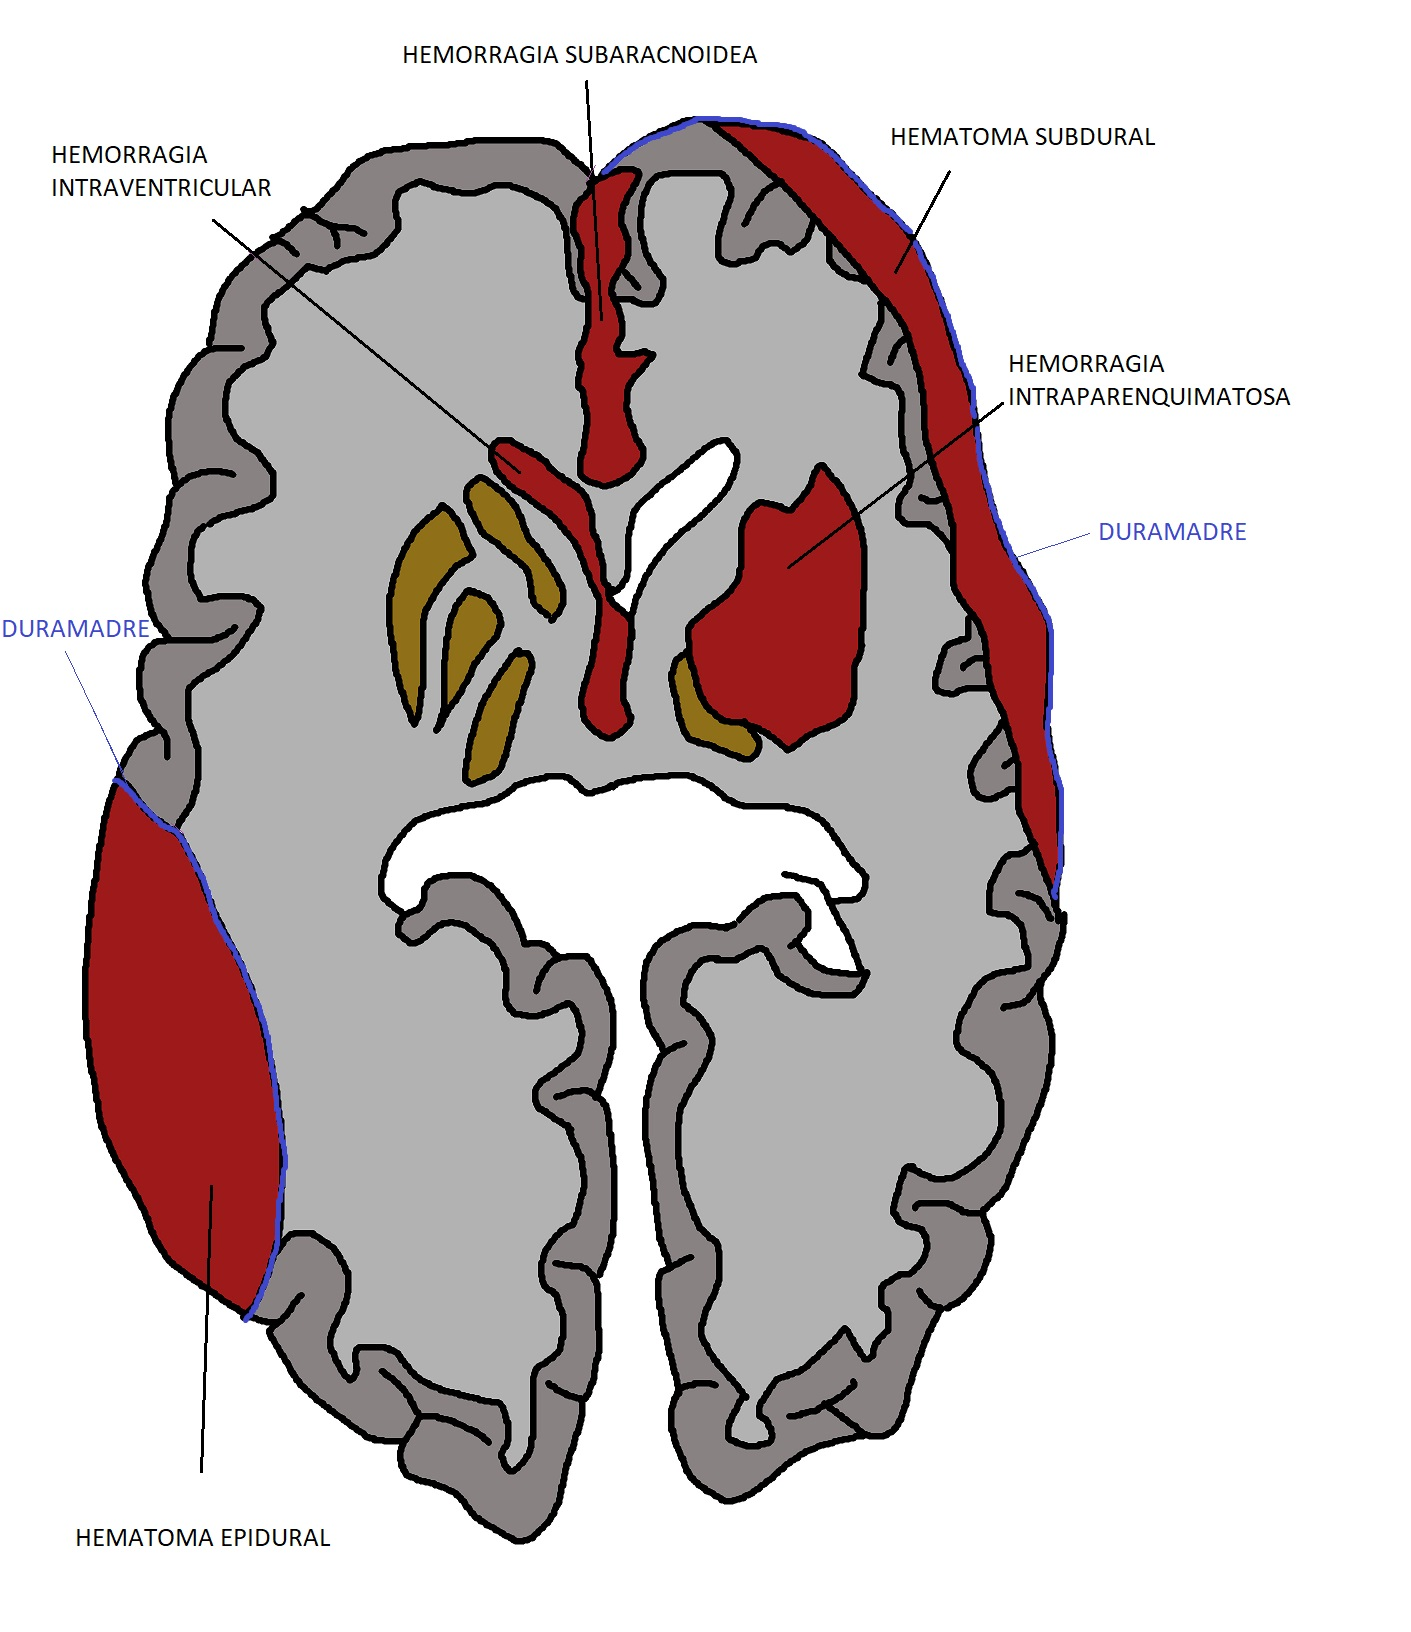
\includegraphics[width=0.7\textwidth]{imagenes/Figura3}
		\caption{Tipos de hematoma y hemorragia según localización.}
		\label{fig:figura3}
	\end{figure} 

	\item Hematoma subdural \ref{fig:figura3}: son hemorragias que aparecen entre la duramadre y la membrana subaracnoidea. A diferencia de los epidurales, que se limitan a la zona de fractura, los subdurales se diseminan sobre el hemisferio cerebral, llenando y manteniendo aperturas en los surcos y formando acúmulos con depresión de la superficie cortical. Su origen suele estar en el desgarro de las venas puente (venas corticales superficiales que drenan hacia los senos durales y perforan la aracnoides antes de entrar en los senos), debido a lesiones por aceleración-deceleración tras el impacto (aunque en el síndrome del niño sacudido no se asocia a impacto). Clínicamente, se manifiesta rápidamente, debido al edema cerebral y a la compresión del tronco del encéfalo, sin embargo, el intervalo lúcido es variable, sobre todo en ancianos, que puede prolongarse. En la autopsia, medir su volumen es importante, ya que 35ml puede producir síntomas neurológicos y, a partir de 50ml (aunque en algunos individuos toleran hasta 100 ml), es ya peligroso para la vida. Se clasifican en agudos, subagudos y crónicos. Si produce síntomas tras el impacto es agudo, si los produce 2-3 semanas después subagudo y, a partir de 3 semanas, crónico. 
	\item Hemorragia subaracnoidea \ref{fig:figura3}: es el segundo indicador más común de lesión traumática encefálica. Sin embargo, si está en pequeña cuantía en la corteza frontoparietal paramediana puede ser difícil de distinguir del artefacto por manipulación en la autopsia. Para evitar este problema, si hay sospecha de traumatismo hay que hacer una inspección de la superficie meníngea con el cerebro in situ, con cuidado durante la retirada de la duramadre. Un indicador de hemorragia antemortem es la congestión hemorrágica oscura en forma de granulaciones sobre la duramadre. Para que produzca la muerte, hace falta un gran volumen de hemorragia, por lo que en casos de baja cantidad el mecanismo etiopatogénico se encuentra en el daño axonal difuso, la lesión hipóxica-isquémica o el edema cerebral. En casos de muerte asociada a un traumatismo craneal, es frecuente encontrar pequeñas cantidades de hemorragia en un área amplia, sin embargo, en ausencia de hemorragia subdural o de lesión axonal difusa, establecer la causa de la muerte puede ser problemático, ya que una pequeña cantidad no es un factor suficiente. Se postula que el mecanismo de muerte puede ser por apnea post-traumática ó aumento de catecolaminas. 
	\item Contusión cerebral: es el marcador de lesión craneal traumática más común. Aparece en forma de moratones hallados en los ápices de los giros, que tienden a localizarse de forma recurrente en zonas concretas. Ocurren en el momento del impacto contra las prominencias óseas suprayacentes. Para distinguirlos de los infartos, hay que tener en cuenta que estos últimos muestran una localización más aleatoria, no se limitan a los ápices de los giros y muestran una preservación relativa de la capa I de la corteza. Se pueden acompañar de hematomas corticales/subcorticales de un volumen variable. Los de mayor tamaño, se introducen en la sustancia blanca subcortical y pueden acabar en un ventrículo adyacente. Las contusiones también suelen asociarse más a fuerzas de aceleración-deceleración, apreciándose correlación entre la fuerza del impacto y la extensión de las contusiones. 
	\item Lesión axonal difusa: lesión de las fibras axonales de la sustancia blanca en un área amplia del cerebro (sin afectar la totalidad del mismo). Estas lesiones en encuentran en relación con fuerzas de aceleración-deceleración y pueden constituir el principal mecanismo etiopatogénico que lleve a la muerte del individuo en casos donde se produzcan este tipo de fuerzas, como en los accidentes de tráfico. 
\end{itemize}

\section{Daño axonal difuso}
\subsection{Concepto} \cite{Davceva2015} \cite{Gaetz2004} \cite{Johnson2013} \cite{Profyris2004} \cite{Stoica2010}
El daño axonal difuso es una entidad clínico-patológica que se caracteriza clínicamente por una pérdida de consciencia inmediata y prolongada tras el impacto mecánico en la cabeza, típicamente sin intervalo lúcido, llevando a daño cerebral severo, estado vegetativo y muerte. Patológicamente, se caracteriza por un daño extendido y diseminado de las fibras axonales de la sustancia blanca, incluyendo tractos nerviosos y tronco del encéfalo.

Aunque la etiología de la lesión axonal difusa es traumática por definición, este término se ha empleado de forma imprecisa para definir patología axonal de cualquier causa. La entidad patológica conocida anteriormente como lesión axonal difusa (DAI) se conoce actualmente como lesión axonal difusa traumática (diffuse TAI). Sin embargo, la entidad clínico-patológica de DAI permanece. De hecho, la definición original de DAI requería historia de traumatismo previo para realizar el diagnóstico, condición que no siempre puede cumplirse en la práctica forense, sea por ausencia de historia definida o por la falta de correlación con las lesiones observadas post-mortem. Para solventar este problema, se establecieron unos patrones de lesión axonal que permiten su interpretación como “altamente sugestivos de traumatismo”, en aquellos casos en los que se carezca de historia definida \cite{Reichard2005}

Los principales mecanismos que juegan un papel clave en las lesiones craneales son en primer lugar el fenómeno de contacto y en segundo lugar las fuerzas de aceleración-deceleración\cite{Gaetz2004}. Esta última, como resultado de un movimiento brusco de la cabeza, provoca gradientes de presión en la cavidad intracraneal, iniciando fuerzas de cizalla y torsión. Estos fenómenos de inercia típicamente producen un hematoma subdural agudo (por la ruptura de vasos sanguíneos) y daño axonal difuso en la sustancia blanca (por torsión y desgarramiento de las fibras axonales) \ref{fig:figura4}

	\begin{figure}
	\centering
	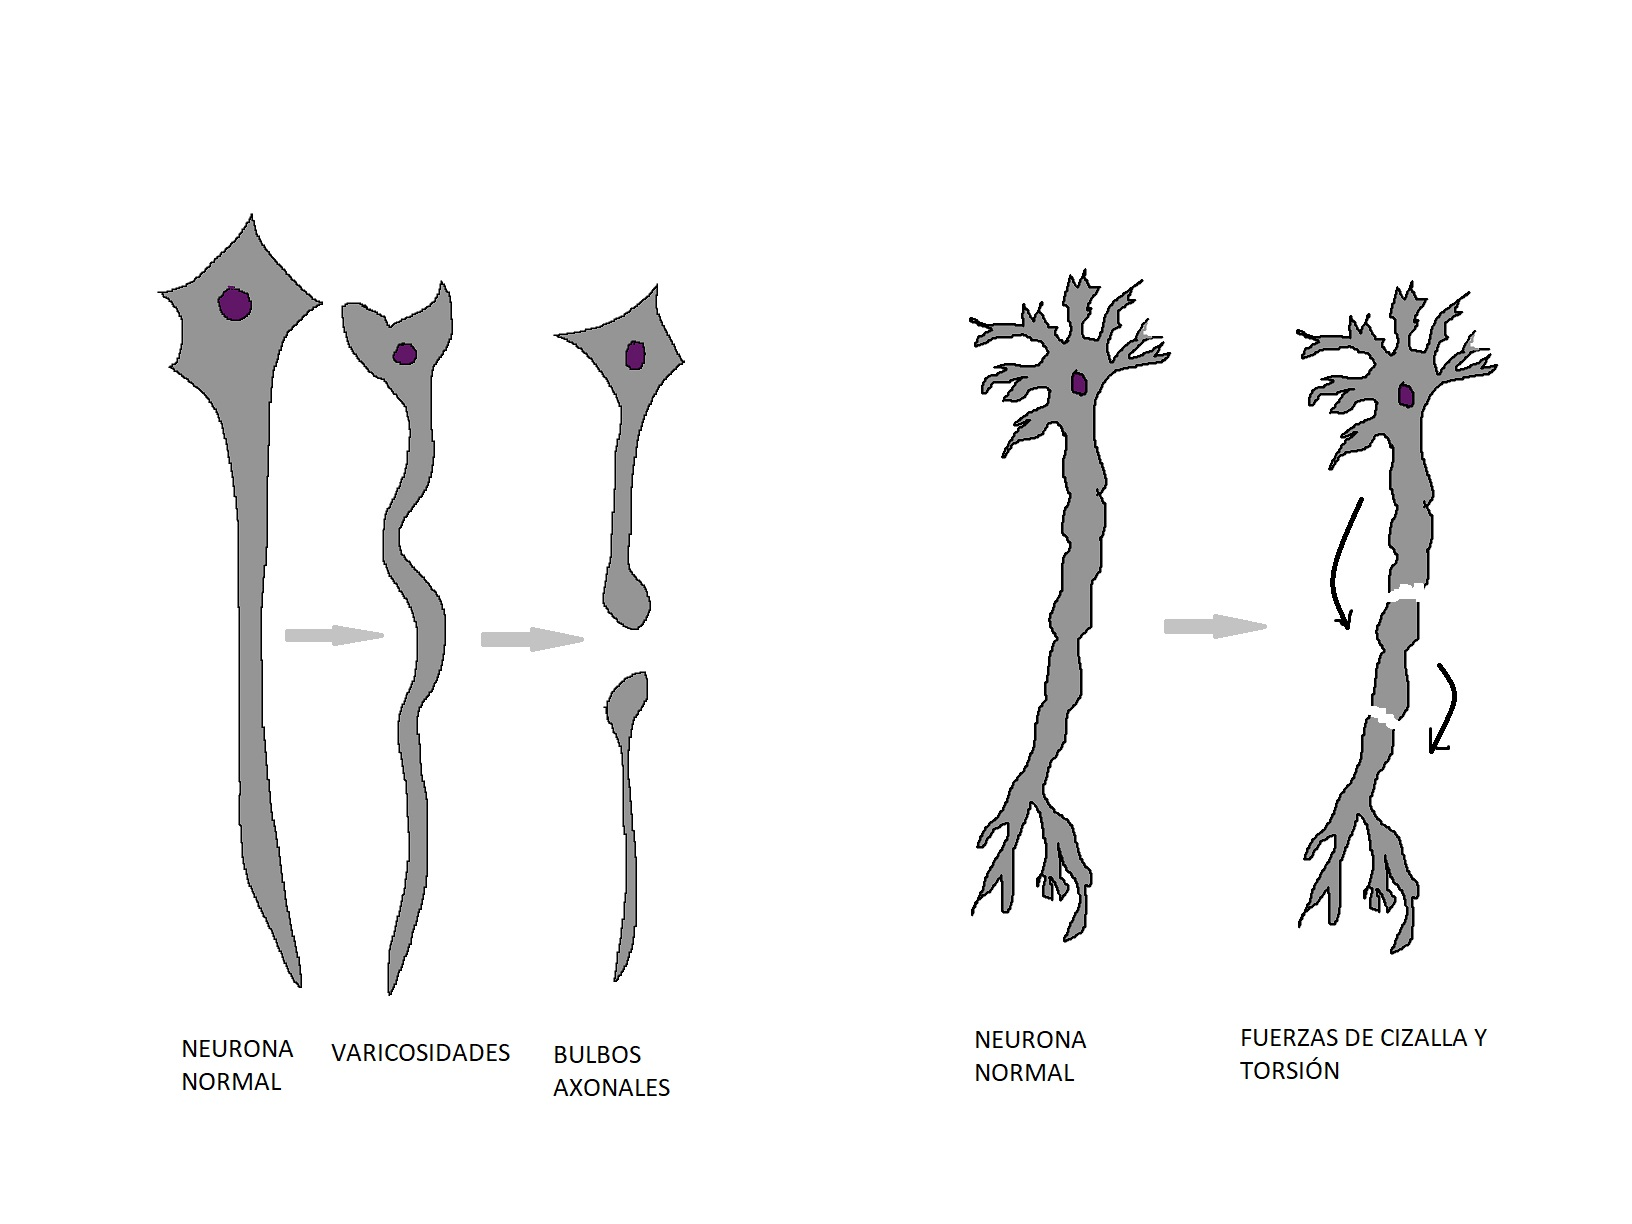
\includegraphics[width=0.7\textwidth]{imagenes/Figura4}
	\caption{A la izquierda, aspecto del axon con varicosidades hasta la formación de bulbos axonales. A la derecha, imagen de neurona afectada por fuerzas de cizalla.}
	\label{fig:figura4}
\end{figure} 

El hematoma subdural se produce en eventos de aceleración angular de corta duración (5-10 milisegundos), como en casos de caída simple o de asalto, mientras que el daño axonal difuso tiene lugar en casos en los que la cabeza se mueve en un plano coronal y la duración de la aceleración es mayor (20-25 milisegundos), con una tasa de aceleración menor, siendo más típico de accidentes de tráfico (no ciclistas) ó caídas desde una altura considerable \cite{Oehmichen1998}

A nivel celular, este impacto inicial produce una perturbación focal del axón, provocando una disrupción del transporte axosplásmico y el acúmulo subsecuente de sustancias que forman parte del axolema - entre ellas la proteína precursora de $\beta$-amiloide – siendo la axotomía primaria un evento raro. La $\beta$-APP es una glicoproteína transmembrana que participa en numerosas funciones fisiológicas celulares. Se sintetiza en el pericarion neuronal, moviéndose posteriormente por transporte anterógrado rápido (100-400mm/día), por lo que en condiciones normales no se acumula lo suficiente como para que pueda detectarse en el tejido. Sin embargo, en caso de daño axonal estructural, se acumula en los segmentos proximales y distales del axón, de tal manera que puede detectarse por medio de técnicas inmunohistoquímicas a partir de 2-3 horas desde el daño inicial4 (Ver tabla 2 y 3) \cite{Hostiuc2014}

La distribución macroscópica \cite{Reichard2005} de daño axonal descrita en relación a trauma incluye el cuerpo calloso (particularmente posterior), la cápsula interna y los pedúnculos cerebelosos. Sin embargo, la lesión axonal en estas ubicaciones puede camuflarse por la lesión axonal secundaria a complicaciones vasculares ó asociada a otras patologías subyacentes (ver tabla Anexo 3). En estos casos, la histología es una herramienta útil, ya que en lesiones de origen traumático los axones tienden a estar dispersos o agrupados, pero confinados a paquetes individuales en la sustancia blanca y, en el daño isquémico, los axones tienden a mostrar un patrón lineal o geográfico, sin delimitar paquetes individuales en la sustancia blanca. No obstante, esta característica no siempre permite una clasificación precisa, ya que las lesiones pueden camuflarse dentro de las complicaciones asociadas a edema cerebral e incremento de la presión intracraneal. Las técnicas inmunohistoquímicas, tales como la aplicación de $\beta$-APP, han constituido un avance a la hora de identificar nuevos patrones que nos permitan una catalogación más fiable, paliando las imprecisiones generadas por efectos secundarios a la lesión principal \cite{Geddes1997} \cite{Graham2004} \cite{Reichard2005} \cite{Traumatic}

En la práctica forense, el reconocimiento de estas lesiones puede implicar una lesión rotacional de considerable gravedad, tales como un accidente de tráfico ó una precipitación, sugiriendo cuál podría ser el principal mecanismo etiopatogénico que ha llevado al fallecimiento del individuo y, por lo tanto, aportando información de interés en aquellos casos en los que se carece de historia previa.

\subsection{Estado del Arte}
Realizado por MacKenzie y FRC Path, en "Axonal Injury in Stroke: A Forensic Neuropathology Perspective" (2015) \cite{MacKenzie2015}, partiendo de la premisa de que la lesión axonal difusa puede tener múltiples causas además del trauma, decidieron definir qué lesiones se observaban en cerebros de personas fallecidas por infarto, para poder buscar rasgos distintivos se seleccionaron 100 casos de infarto, sin historia de lesión craneal, de los archivos del departamento de patología de la Universidad de Aberdeen. Tras las pérdidas, se obtuvo una cohorte de 96 casos, de los cuales 47 eran infartos isquémicos y 49 infartos hemorrágicos. Las secciones de parafina se tiñeron con Luxol Fast Blue/HE, para estudio morfológico y con $\beta$-APP. Se obtuvieron copias de los informes de autopsia para determinar el tiempo de supervivencia desde la aparición de síntomas y signos de infarto, hasta la muerte. El estudio confirmó que, en presencia de isquemia cerebral o hemorragia, el patrón de $\beta$-APP es muy difícil de interpretar y puede simular el mismo patrón que en una lesión cerebral traumática y que la tinción de $\beta$-APP ha de ser interpretada en el contexto de la totalidad de los hallazgos neuropatológicos, no de forma aislada. Acaban concluyendo que es necesaria cierta cautela a la hora de interpretar los hallazgos y crean un pequeño algoritmo que permite aseverar que una lesión es de origen traumático si se cumplen los siguientes: no hay evidencia de edema cerebral macroscópico, no hay evidencia de neuronas isquémicas, palidez de la sustancia blanca o hemorragia en áreas seleccionadas para aplicar la $\beta$-APP y el patrón de la misma no es geográfico (en "zigzag"), sin axones inmunoreactivos en zonas con hemorragia traumática o límites arteriales.\
Realizado por Davceva, Basheska y Balazic, en "Diffuse Axonal Injury- A distinct clinicopathological entity in closed head injuries" (2015) \cite{Davceva2015} hacen una revisión de los hechos conocidos y las cuestiones que aún siguen pendientes con respecto a esta entidad, tanto en diagnóstico (¿hay diferencias entre el daño axonal causado por isquemia y el daño axonal causado por trauma? ¿la isquemia secundaria enmascara el daño axonal traumático? ¿qué se puede concluir con certeza de la apropiada interpretación del daño axonal?) como en su relevancia médico-legal (¿es el daño axonal difuso más característico de ciertos eventos traumáticos?¿Tiene alguna relevancia biomecánica que pueda aportar alguna ventaja al médico forense?¿puede indicar el tipo de evento traumático que ha causado el daño craneal?), remarcando su utilidad actual en el contexto médico-legal y la necesidad de seguir realizando estudios que aporten más datos para responder a las preguntas planteadas. \
Realizado por Reichard, Smith y Graham, “The significance of $\beta$-APP immunoreactivity in forensic practice” (2005) \cite{Reichard2005}, trata de evaluar si las descripciones de distintos patrones morfológicos y distribuciones de la $\beta$-APP se podían emplear microscópicamente para distinguir el daño axonal asociado a trauma de otras causas. Revisaron un total de 73 casos seleccionados de 6 grupos distintos (lesión axonal traumática difusa, infarto cardíaco, hipoglucemia, estatus epiléptico, intoxicación por monóxido de carbono y controles sin alteraciones neuropatológicas). Realizaron 8 cortes de cada muestra y se procesaron para IHQ y HE. Posteriormente, se revisó cada uno de los casos de forma ciega al diagnóstico clínico, realizando un diagnóstico provisional en base a la distribución del daño axonal en la IHQ con $\beta$-APP. En los casos positivos, se procedió a revisar las secciones de HE, realizándose un segundo diagnóstico patológico basado en ambas.  Por último, se compararon los diagnósticos realizados con la historia clínica del caso. Se correlacionaron correctamente un 85 por ciento de los casos y fueron identificadas un 82 por ciento de las lesiones axonales difusas traumáticas. Concluyeron que se pueden emplear los patrones microscópicos de distribución de $\beta$-APP en daño axonal difuso de origen traumático y en lesión isquémica difusa para determinar la causa de la patología axonal y que, por lo tanto, cuando no se dispone de historia clínica, la IHQ puede aportar información útil en relación al tipo de lesión cerebral. 

Realizado por Smith, Meaney, Shull “Diffuse Axonal Injury in Head Trauma” (2003) \cite{Smith2003}, buscaron evaluar la evolución de los patrones de patología axonal en función del tiempo de desarrollo desde el traumatismo inicial. Su idea principal era intentar establecer los mecanismos fisiopatológicos de la misma, en un intento de buscar una correlación clínica-radiológica de tal manera que se pudiera identificar en pacientes vivos e iniciar un tratamiento. 
Realizado por Oehmichen, Meibner, Swchmidt, Pedal, Konig, Satemus “Axonal injury – a diagnostic tool in forensic 1 neuropathology? A review” (1998)\cite{Oehmichen1998}, este grupo detectó la lesión mediante empleo de $\beta$-APP, en un intento de determinar la incidencia, especificidad y significado biomecánico del daño axonal para determinar vitalidad y tiempo de supervivencia. Estudiaron 252 cerebros divididos en lesión fatal de cabeza “cerrada” (incluyendo lesiones sin proyectiles pero excluyendo casos con fractura o impresión craneal; subdividido a su vez en hemorragia cortical fatal, hematoma subdural fatal, o una combinación de ambos), lesión cerebral por proyectil, muerte cerebral (tras lesión inducida mecánicamente, tras lesión no inducida mecánicamente, tras hipoxia/isquemia cerebral global terminal) y shock hemorrágico agudo sin lesión cerebral traumática (grupo control). En todos los casos, estudiaron la $\beta$-APP, considerándola positiva en axones individuales, fragmentos de axones o bulbos axonales detectados de forma repetida en una de las secciones cerebrales. En base a los resultados, establecieron los siguiente:

\begin{enumerate}
	\item La $\beta$-APP es un marcador muy específico de lesión axonal.
	\item La expresión de $\beta$-APP es un indicador de circulación intacta durante el proceso de lesión axonal (muestra de vitalidad). 
	\item La estimación del tiempo de supervivencia valorando el daño axonal difuso es posible mediante la aplicación de distintas técnicas histológicas.
	\item Los procesos físicos y metabólicos pueden inducir expresión de $\beta$-APP focal (no específica). 
	\item Los fenómenos de lesión axonal difusa (DAI), es decir, demostración simultánea de lesión axonal en el cuerpo calloso y en el puente, es un indicador de traumatismo físico (específico). 
	\item Una aceleración rotacional puede inducir daño axonal difuso (trasfondo biomecánico). 
\end{enumerate}
Realizado por Geddes, Vowles, Beer, Ellison, “The diagnosis of diffuse axonal injury: implications for forensic practice” (1997) \cite{Geddes1997}. Al ver la relevancia que podía tener el estudio del daño axonal difuso, pero el trabajo y el gran número de muestras que requería su diagnóstico, este grupo evaluó si era posible disminuir el número de bloques necesarios para realizar el diagnóstico de lesión axonal difusa. Para ello, emplearon una serie de 22 casos previamente diagnosticados, en los que se evaluaron 3 muestras supratentoriales y 3 muestras infratentoriales, teñidas con $\beta$-APP, CD68 y GFAP. El estudio concluyó que un muestreo restringido no permite el diagnóstico fiable de daño axonal difuso, que la detección temprana de $\beta$-APP hay que interpretarla con mucha precaución (en periodos cortos de supervivencia – menores de 24 horas – el dato más relevante es la ausencia de lesión en un cerebro bien muestreado), que en periodos de supervivencia mayores a 24 horas un panel de marcadores IHQ que incluyan $\beta$-APP en combinación con marcadores de microglía como CD68 proporciona medios satisfactorios de diagnosticar daño axonal traumático, incluyendo GFAP en casos de supervivencia más prolongados, y que la data precisa de los cambios histológicos no parece posible.
\subsection{Objetivos del estudio}
\subsubsection{Objetivos generales}
\begin{enumerate}
	\item Identificar lesiones de daño axonal difuso en distintas patologías.
	\item Prevalencia del daño axonal difuso en patología forense de origen traumático, incluyendo ahorcaduras.
	\item Identificar posibles lesiones de daño axonal difuso en casos de elongación cervical. 
	
\end{enumerate}
\subsubsection{Objetivos específicos}
\begin{enumerate}
	\item Identificar necropsias cuya causa de fallecimiento sea por precipitación, tráfico, ahorcadura o que padezcan/se sospeche una de las siguientes: Enfermedad lateral amiotrófica, enfermedad de Huntington, esclerosis múltiple, leucoencefalopatía multifocal progresiva, hipoglucemia, enfermedad de Niemann-Pick tipo C, Déficit vitamina E, embolia, encefalopatía global hipóxico-isquémica, neurotoxinas, radiación.   
	\item Tomar muestra de encéfalo, tronco del encéfalo y porción craneal de la médula espinal de aquellas que cumplan los requisitos anteriores (ver anexo 1).
	\item Estudio de bloques específicos de dichas muestras tras tinción con hematoxilina-eosina. Se busca identificar axones esferoides y, si es posible, neuronas balonizadas degeneradas.
	\item Aplicar $\beta$-APP en cortes seleccionados para caracterización precoz del daño axonal difuso. 
	\item Establecer una relación entre la presencia de daño axonal difuso y las patologías que se han seleccionado previamente.
	\item Establecer posible relación cronológica entre tiempo de supervivencia/data de la muerte y la presencia de daño axonal difuso. 
	
\end{enumerate}
    En todo momento se cumplirá el compromiso de guardar estricta reserva en relación a la información confidencial mediante la oportuna firma de la Cláusula de Confidencialidad, así como de tener una conducta ética durante y después del desempeño de las funciones.
%
%\input{capitulos/02_EspecificacionRequisitos}
%
%\input{capitulos/03_Planificacion}
%
%\input{capitulos/04_Analisis}
%
%\input{capitulos/05_Diseno}
%
%\input{capitulos/06_Implementacion}
%
%\input{capitulos/07_Pruebas}
%
%\input{capitulos/08_Conclusiones}
%
%%\chapter{Conclusiones y Trabajos Futuros}
%
%
%%\nocite{*}
%\bibliography{bibliografia/bibliografia}\addcontentsline{toc}{chapter}{Bibliografía}
%\bibliographystyle{miunsrturl}
%
%\appendix
%\input{apendices/manual_usuario/manual_usuario}
%%\input{apendices/paper/paper}
%\input{glosario/entradas_glosario}
% \addcontentsline{toc}{chapter}{Glosario}
% \printglossary
\chapter*{}
\thispagestyle{empty}

\end{document}
